\documentclass[a4paper]{article}

\usepackage[utf8]{inputenc}
\usepackage[portuges]{babel}
\usepackage{a4wide}
\usepackage{graphicx}
\usepackage{listings}
\usepackage{caption}
\usepackage{subcaption}
\title{Projeto de Programação Orientada aos Objetos\\Grupo 19}
\author{Henrique Pereira (a80261) \and Pedro Moreira (a82364) \and Pedro Ferreira (a81135) }




\begin{document}

\maketitle

\begin{figure}
\centering
\begin{subfigure}{.4\textwidth}
  \centering
  
\includegraphics[width=.3\linewidth]{henrique.png}
  \caption{Henrique Pereira}
\end{subfigure}
\begin{subfigure}{.4\textwidth}
  \centering
  
\includegraphics[width=.3\linewidth]{pedro.png}
  \caption{Pedro Moreira}
\end{subfigure}
\begin{subfigure}{.4\textwidth}
  \centering
  
\includegraphics[width=.3\linewidth]{ferreira.png}
  \caption{Pedro Ferreira}
\end{subfigure}
\end{figure}



\newpage

\tableofcontents

\newpage

\section{Introdução}
\label{sec:intro}

 No contexto da Unidade Curricular Programação Orientada aos Objetos (POO), foi-nos proposto o desenvolvimento de uma aplicação chamada JAVA-Fatura. 
 Tal como o nome indica, o enunciado proposto pelos docentes visa o desenvolvimento de uma versão da plataforma E-Fatura, de consulta e emissão de faturas, na linguagem \texit{Java}.
 Os requisitos básicos são, por exemplo, por parte do contribuinte individual, verificar as faturas 
 emitidas em seu nome e, por parte de uma empresa, obter o total faturado.
 Na seção \ref{sec:java} serão apresentados mais requisitos desta aplicação e também serão discutidas as classes 
 criadas para a concretização dos requisitos apresentados.
 Na seção \ref{sec:funcionalidades} será discutida a forma como os utilizadores podem interagir com a aplicação.


\section{JAVA-Fatura}
\label{sec:java}

A aplicação teria que permitir, além da criação de novos contribuintes e empresas no sistema, de fazer a identificação correta da entidade que se encontra a utilizar o Java-Fatura, isto é, teria que ser capaz de efetuar o Login no Sistema com sucesso, perante as credenciais dadas.
Para além dos requisitos já referidos, os contribuintes individuais devem ser capazes de verificar o montante de dedução fiscal acumulado (por si
e pelo agregado familiar) e atribuir ou corrigir o setor de atividade económica de uma fatura, sendo que esta alteração teria que ser mantida em registo. 
As empresas deverão ser capazes de de obter
vários tipos de listagens sobre as faturas que emitiram, ordenadas por valor ou data. Para além disso, a aplicação necessita de ter um admistrador capaz 
de determinar os contribuintes que mais gastam no sistema e as empresas que mais faturaram ou de adicionar um novo setor de ativividade económica. Para a realização deste projeto, decidimos
criar as classes que descrevemos na secção \ref{sec:classes}.
}
	

%%%%%%%%%%%%%%%%%%%%%%%%%%%%%%%%%%%%%%%%%%%%%
\subsection{Classes}
\label{sec:classes}

Antes de iniciarmos a descrição de cada uma das classes, começamos por mostrar o diagrama das classes implementadas (pelo \textit{BLUEJ}).

	% IMAGEM 
	
\subsubsection{BeneficioFiscal} %%%%%%%%%%%%%%%%%


Interface definida para que as famílias numerosas e as empresas do interior
possam ter um beneficio fiscal aquando da dedução das suas faturas.
Esta interface contém o método reducaoImposto não definido.


\subsubsection{ConcelhosInterior} %%%%%%%%%%%%%%%

Classe que contém os concelhos que podem usufruir de beneficio fiscal. Pelo facto de serem imensos, decidimos optar por selecionar apenas nove concelhos abrangidos por este benefício, entre eles Penalva do Castelo, Vinhais, Resende, Ribeira de Pena, Baião, Celorico de Bastos, Tabuaço, Cinfães e Mirandela.

Possui apenas uma variável de instância: um mapa que associa a cada concelho do interior a sua taxa de dedução.


\subsubsection{Contribuinte} %%%%%%%%%%%%%%%

Sendo subclasse de Entidade, esta classe tem como variáveis de instância a lista das faturas emitidas em seu nome (separadas pelas que são 
fiscalmente válidas ou inválidas/pendentes) e o número de dependentes familiares e os seus NIF's.


\subsubsection{ContribuinteFamiliaNumerosa} %%%%%%%%%%%%%%%

Implementa a interface BeneficioFiscal e é subclasse de Contribuinte. É aqui que definimos a taxa de benefício fiscal das famílias numerosas e o bónus fiscal que cada dependente representa.


\subsubsection{Controller} %%%%%%%%%%%%%%%

Classe intermediária entre a comunicação do utilizador com o sistema. É lá que está definida a \textit{main} e as funções que nos permitem interagir com os menus por nós criados, e apresentados pelo terminal. A variável de instância que representa o estado do Sistema é criada aqui.


\subsubsection{Distritos} %%%%%%%%%%%%%%%

Enum contendo todos os dezoito distritos do país.


\subsubsection{Empresa} %%%%%%%%%%%%%%%

Subclasse de Entidade que contém as faturas emitidas e os setores de atividade económica. É nesta classe que estão definidos os métodos que permitem a ordenação das faturas, assim como a inserção destas no sistema.


\subsubsection{EmpresaInterior} %%%%%%%%%%%%%%%

Subclasse de Empresa que implementa a interface BeneficioFiscal. É com esta classe que permitimos que os bónus fiscais sejam atribuidos às empresas do interior do país, isto é, cuja atividade está declarada como sendo efetuada num dos concelhos considerados pelo Sistema como sendo do Interior.


\subsubsection{Entidade} %%%%%%%%%%%%%%%

Classe que contém as informações básicas das entidades do sistema, tais como o nome, o email e a morada, assim como as credenciais necessárias para o login (NIF e password).


\subsubsection{Fatura} %%%%%%%%%%%%%%%

Classe onde são guardadas as informações de cada fatura, isto é, o nome e o NIF da empresa, a data de emissão da fatura, o NIF do cliente e a descrição e valor da fatura. Além disso, é também guardado o setor de atividade económica atribuído e o registo de alteração deste. 


\subsubsection{GestorSetor} %%%%%%%%%%%%%%%

Classe auxiliar à classe Fatura para que seja possível ao Contribuinte associar o setor de atividade económica que deseja à fatura em causa. Além disso, permite também saber qual a taxa de dedução fiscal associado a cada Setor, além de permitir também que sejam adicionados novos setores de atividade ao sistema.


\subsubsection{LogSetor} %%%%%%%%%%%%%%%

Classe auxiliar à classe GestorSetor que guarda o histórico de todas as alterações do setor de atividade económica que um contribuinte realizou. Contém ainda informações relativas ao setor ativo.

 
\subsubsection{Menu} %%%%%%%%%%%%%%%

Classe que faz o display das operações que o utilizador pode realizar, isto é, mostra-nos as operações possíveis nos diferentes Menus: inicial, contribuinte, empresa ou administrador.


\subsubsection{Morada} %%%%%%%%%%%%%%%

Classe que permite agregarmos todas as informações relativas à morada de uma entidade, facilitando assim o seu manuseamento. É aqui que representamos a rua, o código postal, o concelho e o distrito de uma entidade.


\subsubsection{Setor} %%%%%%%%%%%%%%%

Classe que contém as informações sobre a dedução relacionada com o setor de atividade económica, ou seja, as taxas de dedução, se as despesas relacionadas com esse setor são dedutíveis e, se assim forem, qual o máximo valor dedutível.


\subsubsection{Sistema} %%%%%%%%%%%%%%%

Classe que guarda todas as informações da aplicação (dados de todas as entidades). Assim sendo, definimos aqui um HashMap com todas as entidades do sistema, um GestorSetor e as informações relativas às credenciais de admnistrados, que são as seguintes:

\textbf{NIF}: \texttt{20172018}

\textbf{Password}: \texttt{miei}



%%%%%%%%%%%%%%%%%%%%%%%%%%%%%%%%%%%%%%%%%%%%%
\subsection{Classes de Exceção}
\label{exceptions}

  \begin{itemize}
  	\item{AdminModeNaoAtivadoException - } 
    \item{ConcelhoNaoEInteriorException - } 
    \item{EntidadeAtivaNaoEEmpresaException - } 
    \item{NIFDaFaturaEEmpresaException - }
    \item{NIFJaRegistadoException - } 
    \item{NIFNaoEDeUmContribuinteException - }
    \item{NIFNaoRegistadoException - }
  \end{itemize}


%%%%%%%%%%%%%%%%%%%%%%%%%%%%%%%%%%%%%%%%%%%%%
\subsection{Decisões Tomadas}
\label{sec:decisoes}

Modelo MVC
GestorSetor



%%%%%%%%%%%%%%%%%%%%%%%%%%%%%%%%%%%%%%%%%%%%%
\subsection{Funcionalidades}
\label{sec:funcionalidades}

Qualquer utilizador quando inicia a aplicação é confrontado com o seguinte menu:

	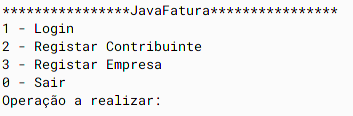
\includegraphics[width=.6\linewidth]{main_menu.png}

Caso o utilizador escolha efetuar o login (1) e o efetue com sucesso (mediante registo prévio no sistema)
o menu seguinte será diferente para cada uma das entidades apresentadas abaixo.
Ao registar, quer um contribuinte, quer uma empresa, serão pedidas informações relativas a cada uma das entidades.


\subsubsection{Contribuinte}

	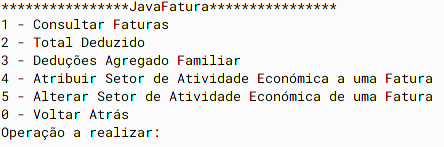
\includegraphics[width=.7\linewidth]{contribuinte_menu.png}


\subsubsection{Empresa}

	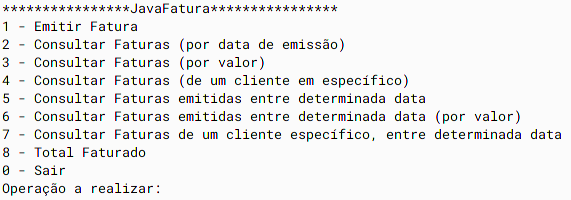
\includegraphics[width=.9\linewidth]{empresa_menu.png}


\subsubsection{Admistrador}

	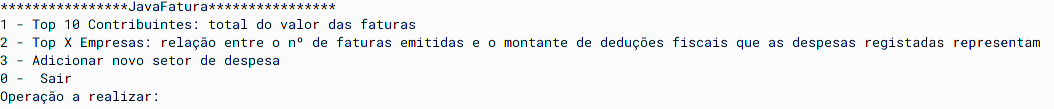
\includegraphics[width=.9\linewidth]{admin_menu.png}




\section{Conclusões}
\label{sec:conclusao}

Este projeto foi extremamente enriquecedor para o grupo, uma vez que nos permitiu pôr em prática os conhecimentos adquiridos nas aulas de POO e desenvolver uma aplicação em JAVA, tendo em conta as orientações dadas pelos docentes no que diz respeito a Programação Orientada aos Objetos. 

Em suma, na nossa opinião, os requisitos propostos foram cumpridos e conjugados com êxito, sendo que o resultado final se revela bastante apelativo e funcional.

Foi, no geral, um trabalho  altamente pedagógico, que nos permitiu desenvolver não só competências essenciais ao curso de Mestrado Integrado em Engenharia Informática, como também competências sociais, tais como o trabalho em grupo.

\end{document}\grid
